\subsection*{MEDUSA: Multi-scale Encoder-Decoder Self-Attention Deep Neural Network Architecture for Medical Image Analysis}

% \subsection*{Ссылка} \url{https://arxiv.org/abs/2110.06063}
\subsection*{Введение}

Анализ медицинских изображений попрежнему сопряжен с трудностями, 
учитывая трудноразличимые грани между заболеваниями с похожими проявлениями, 
что увеличивает важность наличия качественной дифференциальной диагностики.
В данной работе исследуется концепция self-attention для повышения точности 
диагностики, особенно на ранних стадиях развития болезни.
\subsection*{Основная идея}
Авторы предполагают \cite{ann17}, что внедрение явного глобального контекста среди выборочного 
внимания на разных уровнях абстракций в нейросетевой архитектуре при способности различать 
локальный контекст на отдельных уровнях может привести к лучшей производительности.
Чтобы проверить предположение, предлагается MEDUSA (Multi-scale Encoder-Decoder Self-Attention) - 
self-attention механизм, приспособленный для задачи анализа медицинских изображений,
который явно использует связи между глобальным и масштабно-зависимым локальным контекстами 
с помощью реализации \glqq single body, multi-scale heads\grqq для повышения производительности.

\begin{minipage}{1.0\linewidth}
    \begin{center}
        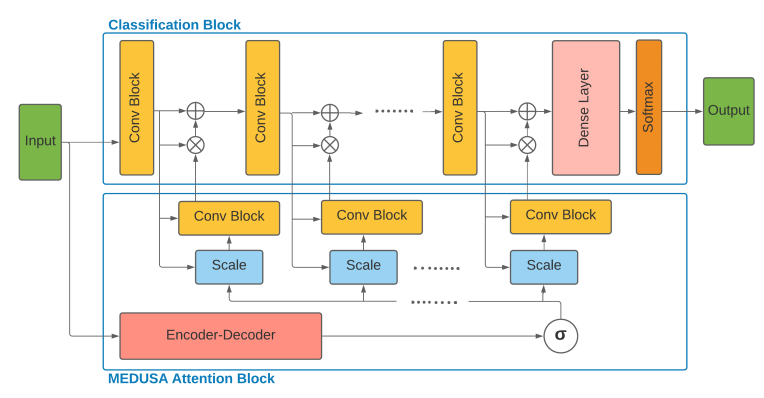
\includegraphics[scale=0.6]{ann17_arch.png} \\
        % \caption{\scriptsize{
        %     Архитектура MEDUSA.
        % }}
    \end{center}
    
\end{minipage} 

\subsection*{Данные}
CXR-2 Dataset
\subsection*{Результаты}
\begin{minipage}{1.0\linewidth}
    \begin{center}
        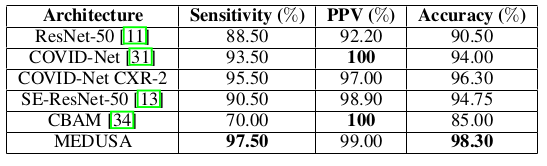
\includegraphics[scale=0.6]{ann17_res.png} \\
        % \caption{\scriptsize{
        %     Sensitivity, PPV - positive predictive value и точность предложенного метода MEDUSA 
        %     в сравнении с другими сетями на данных из CXR-2 Dataset.
        % }}
    \end{center}
    
\end{minipage} 
\subsection*{Заключение}
Было показано, что предложенный метод показывает хорошие результаты как в предсказаниях так и в скорости в сравнении с 
уже существующими моделями.